\documentclass[11pt,a4paper]{article}
\usepackage[margin=2.3cm]{geometry}
\usepackage[T1]{fontenc}
\usepackage{lmodern}
\usepackage{microtype}
\usepackage{amsmath,amssymb,amsthm}
\usepackage{algorithm}
\usepackage{algpseudocode}
\usepackage{booktabs}
\usepackage{graphicx}
\usepackage{float}
\usepackage{xcolor}
\usepackage{enumitem}
\usepackage{tikz}
\usetikzlibrary{arrows.meta,positioning}
\usepackage[hidelinks]{hyperref}
\usepackage[capitalise,noabbrev]{cleveref}
\setlist{itemsep=2pt,topsep=4pt}
\setlength{\emergencystretch}{3em}

\newtheorem{theorem}{Theorem}
\newtheorem{lemma}[theorem]{Lemma}
\newtheorem{corollary}[theorem]{Corollary}
\theoremstyle{definition}
\newtheorem{definition}[theorem]{Definition}
\newtheorem{remark}[theorem]{Remark}

\newcommand{\dd}{\mathit{d}}
\newcommand{\pred}{\pi}
\newcommand{\Ot}{\tilde{O}}
\graphicspath{{../figures/}}

\begin{document}

%======================================================================
\begin{titlepage}
\centering
{\large Shiv Nadar Institution of Eminence\par}
{\large Department of Computer Science and Engineering\par}
\vspace{0.6cm}
{\Large CSD319: Design and Analysis of Algorithms\par}
{\large End-Term Project Report\par}
\vspace{2.2cm}
{\huge\bfseries Breaking the Bellman--Ford Barrier\par}
\vspace{0.4cm}
{\Large Efficient Shortest-Path Algorithms for Graphs\\ with Negative Edge Weights\par}
\vspace{0.6cm}
{\large Problem 2: Shortest-Path Algorithms for Graphs with Negative Edge Weights\par}
\vspace{2.2cm}
\begin{tabular}{ll}
\toprule
\textbf{Name} & \textbf{Roll Number}\\
\midrule
Pragun Kathuria & 2410110237\\
Amitoj Oberoi & 2410110046\\
Tanvi Pandey & 2410110356\\
Vishnu Sriram & 2410110629\\
\bottomrule
\end{tabular}
\vfill
{\large November 2026\par}
\end{titlepage}

%======================================================================
\begin{abstract}
\noindent
We study the single-source shortest-path (SSSP) problem on directed graphs whose edge weights may be negative, together with the closely related task of detecting and certifying negative-weight cycles. We present the classical Bellman--Ford algorithm and prove its correctness and its $\Theta(nm)$ running time, then analyse a sequence of improvements: early termination, Yen's two-DAG ordering (at most $\lceil n/2\rceil$ passes), the randomized ordering of Bannister and Eppstein, the queue-based label-correcting method (SPFA), and Johnson's reweighting technique for all-pairs shortest paths. We prove that every cycle in the predecessor graph of a label-correcting algorithm is negative, which yields cheap, verifiable negative-cycle certificates that can be checked periodically at amortized $O(1)$ cost per relaxation. Combining these ideas, we engineer a \emph{hybrid} variant (BFS-ordered Yen passes, early termination, and amortized certificate checks) that keeps the $\lceil n/2\rceil+1$ worst-case pass bound while detecting negative cycles orders of magnitude sooner than textbook Bellman--Ford. All algorithms are implemented in Python, validated against Floyd--Warshall on thousands of random graphs, and benchmarked on four graph families. Finally we survey the theoretical breakthroughs that broke the decades-old $O(nm)$ barrier: Goldberg's scaling algorithm, the near-linear randomized algorithm of Bernstein, Nanongkai and Wulff-Nilsen (2022) and its refinement by Bringmann, Cassis and Fischer (2023), and Fineman's (2024) first strongly-polynomial improvement for real weights. We close with the main open problems.
\end{abstract}

\tableofcontents
\newpage

%======================================================================
\section{Introduction}

Shortest paths are among the most fundamental problems in algorithm design. When all edge weights are non-negative, Dijkstra's algorithm solves SSSP in $O(m + n\log n)$ time. Many applications, however, naturally produce \emph{negative} weights:

\begin{itemize}
\item \textbf{Currency arbitrage.} With edge weight $-\log r_{uv}$ for exchange rate $r_{uv}$, a negative cycle is exactly a profitable sequence of trades.
\item \textbf{Systems of difference constraints} $x_v - x_u \le c_{uv}$, used in scheduling and timing analysis, are feasible iff the constraint graph has no negative cycle, and shortest-path distances give a feasible solution.
\item \textbf{Minimum-cost flow and assignment.} Residual graphs contain negative-cost edges; potentials computed by negative-weight SSSP make the remaining computations Dijkstra-friendly.
\item \textbf{Subroutines} in all-pairs shortest paths (Johnson), minimum mean cycle, and many scaling algorithms.
\end{itemize}

Negative weights break Dijkstra's greedy invariant (\cref{fig:dijkstra}), and negative cycles make ``shortest path'' ill-defined. For decades the best general algorithm remained Bellman--Ford at $O(nm)$, one of the most famous barriers in graph algorithms. This report (i) formalises the problem, (ii) presents and proves the classical algorithms and practical improvements, (iii) analyses their complexity, (iv) evaluates them experimentally, and (v) surveys the recent theoretical breakthroughs and open gaps.

\begin{figure}[H]
\centering
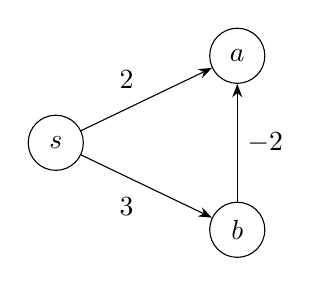
\begin{tikzpicture}[>=Stealth, node distance=2.2cm, every node/.style={circle,draw,minimum size=7mm}]
\node (s) {$s$};
\node (a) [above right=0.6cm and 1.8cm of s] {$a$};
\node (b) [below right=0.6cm and 1.8cm of s] {$b$};
\draw[->] (s) -- node[draw=none,above left,inner sep=1pt]{$2$} (a);
\draw[->] (s) -- node[draw=none,below left,inner sep=1pt]{$3$} (b);
\draw[->] (b) -- node[draw=none,right,inner sep=1pt]{$-2$} (a);
\end{tikzpicture}
\caption{Dijkstra finalises $a$ with distance $2$ before scanning $b$, but the true distance is $3-2=1$.}
\label{fig:dijkstra}
\end{figure}

%======================================================================
\section{Problem Statement}

\begin{definition}[SSSP with negative weights]
\textbf{Input:} a directed graph $G=(V,E)$ with $n=|V|$, $m=|E|$, a weight function $w:E\to\mathbb{R}$ (possibly negative) and a source $s\in V$.\\
\textbf{Output:} either
\begin{enumerate}[label=(\alph*)]
\item the shortest-path distance $\delta(s,v)$ for every $v\in V$ (with $\delta(s,v)=\infty$ if $v$ is unreachable) together with a shortest-path tree, or
\item a \emph{negative cycle certificate}: a cycle $C$ reachable from $s$ with $w(C)=\sum_{e\in C}w(e)<0$.
\end{enumerate}
\end{definition}

If a negative cycle is reachable from $s$, then for every vertex $v$ reachable from that cycle $\delta(s,v)=-\infty$, so case (b) is the only meaningful answer. Negative cycles not reachable from $s$ do not affect the answer and must be ignored. We write $\delta(v)$ for $\delta(s,v)$. When weights are integers we let $W$ (or $N$) denote the largest absolute value of a negative weight; bounds depending on $\log W$ are called \emph{weakly} polynomial and bounds depending only on $n,m$ \emph{strongly} polynomial.

\paragraph{Goals of the project.} (1) Explain the limitations of existing shortest-path algorithms in the presence of negative weights; (2) prove correctness and analyse the complexity of Bellman--Ford and its improvements; (3) investigate opportunities to improve efficiency while still correctly identifying negative cycles, both in practice (implementation and experiments) and in theory (survey of state-of-the-art).

%======================================================================
\section{Background and Related Work}

\begin{table}[H]
\centering
\small
\begin{tabular}{@{}lll@{}}
\toprule
\textbf{Year} & \textbf{Result} & \textbf{Time bound}\\
\midrule
1956--58 & Shimbel; Ford; Bellman; Moore & $O(nm)$\\
1959 & Dijkstra (non-negative weights only) & $O(m+n\log n)$\\
1970 & Yen: two-DAG ordering & $\approx nm/2$ relaxations\\
1977 & Johnson: reweighting for all pairs & $O(nm + n^2\log n)$\\
1981 & Tarjan: subtree disassembly for cycle detection & $O(nm)$\\
1983--89 & Gabow; Gabow--Tarjan: scaling & $O(n^{3/4} m\log W)$, $O(\sqrt n\, m\log(nW))$\\
1995 & Goldberg: scaling & $O(\sqrt n\, m\log W)$\\
2012 & Bannister--Eppstein: random ordering & $\approx nm/3$ relaxations (expected)\\
2022 & Chen et al.: almost-linear min-cost flow (implies SSSP) & $m^{1+o(1)}\log W$\\
2022 & Bernstein--Nanongkai--Wulff-Nilsen (FOCS best paper) & $O(m\log^8 n\log W)$\\
2023 & Bringmann--Cassis--Fischer & $O(m\log^2 n\log(nW)\log\log n)$\\
2024 & Fineman: first strongly-polynomial improvement & $\Ot(mn^{8/9})$\\
2025 & Huang--Jin--Quanrud & $\Ot(mn^{4/5})$\\
\bottomrule
\end{tabular}
\caption{Milestones for SSSP with negative weights. Results from 2022 onward are randomized (Las Vegas or high probability), and the $\log W$ bounds assume integer weights.}
\label{tab:history}
\end{table}

All classical algorithms are \emph{label-correcting}: they maintain tentative distances $\dd(v)\ge\delta(v)$ and repeatedly \emph{relax} edges. The modern algorithms combine \emph{scaling} (reduce the problem to weights $\ge -1$) with graph decompositions and Dijkstra-like phases; we sketch them in \cref{sec:modern}.

%======================================================================
\section{Algorithms}

\subsection{The relaxation framework}

Every algorithm keeps $\dd(v)$ and a predecessor pointer $\pred(v)$. Initially $\dd(s)=0$, $\dd(v)=\infty$ otherwise and $\pred(v)=\textsc{nil}$.

\begin{algorithm}[h]
\caption{\textsc{Relax}$(u,v)$}
\begin{algorithmic}[1]
\If{$\dd(u)+w(u,v) < \dd(v)$}
  \State $\dd(v)\gets \dd(u)+w(u,v)$; \quad $\pred(v)\gets u$
\EndIf
\end{algorithmic}
\end{algorithm}

The algorithms differ only in \emph{which} edges they relax and in \emph{what order}, and in how they recognise that a negative cycle exists.

\subsection{Bellman--Ford (with early termination)}

\begin{algorithm}[h]
\caption{\textsc{Bellman-Ford}$(G,w,s)$}
\label{alg:bf}
\begin{algorithmic}[1]
\State initialise $\dd,\pred$
\For{$i=1$ \textbf{to} $n-1$}
  \State $\mathit{changed}\gets$ \textbf{false}
  \For{each edge $(u,v)\in E$} \State \textsc{Relax}$(u,v)$; set $\mathit{changed}$ if $\dd(v)$ decreased \EndFor
  \If{\textbf{not} $\mathit{changed}$} \Return $(\dd,\pred)$ \Comment{early termination}\EndIf
\EndFor
\For{each edge $(u,v)\in E$}
  \If{$\dd(u)+w(u,v)<\dd(v)$} \Return \textsc{ExtractCycle}$(\pred)$ \Comment{negative cycle}\EndIf
\EndFor
\State \Return $(\dd,\pred)$
\end{algorithmic}
\end{algorithm}

The textbook version always performs $n-1$ passes; the early-termination test stops as soon as a pass changes nothing. If a negative cycle is reachable, no pass ever ``converges'', so the algorithm runs all $n$ passes before detecting it.

\subsection{Yen's ordering and its randomized variant}

Fix a linear order (ranking) of the vertices. Split $E$ into \emph{forward} edges $E_f=\{(u,v): \mathrm{rank}(u)<\mathrm{rank}(v)\}$ and \emph{backward} edges $E_b$. Both $(V,E_f)$ and $(V,E_b)$ are DAGs whose topological orders are the ranking and its reverse. A \emph{Yen pass} relaxes the edges of $E_f$ in increasing rank of their tails, then the edges of $E_b$ in decreasing rank of their tails. Yen (1970) showed that $\lceil n/2\rceil$ passes suffice (\cref{thm:yen}), halving the work of Bellman--Ford. Bannister and Eppstein (2012) showed that choosing the ranking \emph{uniformly at random} reduces the expected number of relaxations further, to about $nm/3$.

\subsection{Queue-based Bellman--Ford (SPFA)}

Instead of relaxing every edge in every pass, keep a FIFO queue of vertices whose label decreased since they were last scanned, and relax only their out-edges:

\begin{algorithm}[h]
\caption{\textsc{SPFA}$(G,w,s)$}
\label{alg:spfa}
\begin{algorithmic}[1]
\State initialise $\dd,\pred$; $Q\gets\langle s\rangle$; $\mathit{cnt}(v)\gets 0$ for all $v$
\While{$Q\neq\emptyset$}
  \State $u\gets Q.\textsc{pop}()$; $\mathit{cnt}(u)\gets\mathit{cnt}(u)+1$
  \If{$\mathit{cnt}(u)\ge n$} \State negative cycle detected (\cref{lem:spfa}) \EndIf
  \For{each $(u,v)\in E$}
     \If{\textsc{Relax}$(u,v)$ decreased $\dd(v)$ \textbf{and} $v\notin Q$} $Q.\textsc{push}(v)$\EndIf
  \EndFor
\EndWhile
\end{algorithmic}
\end{algorithm}

SPFA has the same $O(nm)$ worst case but is often far faster on random inputs, because it only touches ``active'' parts of the graph.

\subsection{Negative-cycle certificates from the predecessor graph}

The \emph{predecessor graph} $G_\pred$ has an edge $(\pred(v),v)$ for each $v$ with $\pred(v)\neq\textsc{nil}$. Every vertex has in-degree at most one in $G_\pred$, so a cycle can be found in $O(n)$ time by following pointers with three-colour marking. \Cref{lem:predcycle} shows that \emph{any} cycle in $G_\pred$ is a negative cycle in $G$. This gives an inexpensive, verifiable certificate.

\paragraph{Amortized checking (Cherkassky and Goldberg, 1999).} Searching $G_\pred$ after every $\Theta(n)$ label updates (or after every pass) costs $O(n)$ per check, i.e.\ $O(1)$ amortized per relaxation, and detects a negative cycle as soon as one appears in $G_\pred$, typically long before the $n$ passes Bellman--Ford needs.

\paragraph{Extracting the cycle in Bellman--Ford.} When the extra pass of \cref{alg:bf} still relaxes an edge, we keep relaxing and search $G_\pred$ until it contains a cycle; this is guaranteed to happen after finitely many further relaxations (Cherkassky and Goldberg, 1999), and the cycle found is negative by \cref{lem:predcycle}.

\subsection{Our hybrid variant}

Our implementation combines three ideas that are each individually justified:
\begin{enumerate}
\item \textbf{Yen passes with a BFS ranking.} We rank vertices in breadth-first order from $s$ (computed in $O(n+m)$). Shortest paths tend to move away from $s$, so most of their edges are forward edges and long monotone runs are fixed within a single half-pass. Since \cref{thm:yen} holds for \emph{every} ranking, the worst case is still $\lceil n/2\rceil+1$ passes.
\item \textbf{Early termination} after a pass with no change.
\item \textbf{A predecessor-graph cycle check after every pass} ($O(n)$ per pass of cost $\Theta(m)$), returning a certificate as soon as one exists.
\end{enumerate}

\subsection{Johnson's algorithm for all pairs}

Add a new vertex $q$ with zero-weight edges $(q,v)$ for all $v$, run Bellman--Ford from $q$ to obtain $h(v)=\delta(q,v)$ (or a negative cycle), reweight every edge as $\hat w(u,v)=w(u,v)+h(u)-h(v)\ge 0$, and run Dijkstra from every vertex. Distances are recovered as $\delta(u,v)=\hat\delta(u,v)-h(u)+h(v)$.

\subsection{Beyond Bellman--Ford: scaling and near-linear algorithms}
\label{sec:modern}

\paragraph{Goldberg's scaling algorithm (1995).} For integer weights $\ge -N$, the algorithm processes the bits of the weights from most to least significant. At each scale the problem reduces to finding a \emph{potential} $p$ that makes all reduced weights $w_p(u,v)=w(u,v)+p(u)-p(v)\ge 0$ when the current weights are all $\ge -1$. Goldberg shows how to eliminate a $\sqrt n$ fraction of the negative vertices per round by working on the strongly connected components and layers of the \emph{admissible} graph (edges of reduced weight $\le 0$), so that each scale costs $O(\sqrt n\, m)$ and the total is $O(\sqrt n\, m\log N)$.

\paragraph{Bernstein--Nanongkai--Wulff-Nilsen (2022).} The first near-linear algorithm, $O(m\log^8 n\log W)$ with high probability. It also uses scaling: a procedure \textsc{ScaleDown} turns weights $\ge -2B$ into weights $\ge -B$. Inside, the graph with weights shifted by $+B$ is broken by a \emph{low-diameter decomposition} into strongly connected pieces of small weak diameter, with each edge cut only with small probability. Pieces are handled recursively, edges between pieces form a DAG that is fixed in one topological sweep, and remaining negative edges are eliminated by a Dijkstra/Bellman--Ford hybrid whose cost is proportional to the average number of negative edges on shortest paths, which the decomposition keeps small.

\paragraph{Bringmann--Cassis--Fischer (2023).} A simpler and faster version, $O(m\log^2 n\log(nW)\log\log n)$, using a new decomposition and a refined analysis of the hybrid Dijkstra step.

\paragraph{Real weights: Fineman (2024) and successors.} Scaling needs integer weights. For arbitrary real weights, Fineman gave the first algorithm beating $O(nm)$ in over six decades, $\Ot(mn^{8/9})$ randomized, by repeatedly ``neutralising'' sets of negative vertices using hop-limited reachability arguments. Huang, Jin and Quanrud (2025) improved this to $\Ot(mn^{4/5})$.

%======================================================================
\section{Proof of Correctness}
\label{sec:proofs}

Throughout, $\delta(v)=\delta(s,v)$, and ``a pass'' means relaxing every edge of $E$ once, in some order.

\begin{lemma}[Upper-bound invariant]\label{lem:upper}
For any sequence of relaxations, $\dd(v)\ge\delta(v)$ for all $v$ at all times, and whenever $\dd(v)<\infty$ there is a walk from $s$ to $v$ of weight $\dd(v)$.
\end{lemma}
\begin{proof}
Induction on the number of relaxations. Initially $\dd(s)=0$ (the empty walk) and all other labels are $\infty$. If \textsc{Relax}$(u,v)$ sets $\dd(v)=\dd(u)+w(u,v)$, then by induction there is an $s$--$u$ walk of weight $\dd(u)$; appending $(u,v)$ gives an $s$--$v$ walk of weight $\dd(v)$, and every walk weighs at least $\delta(v)$.
\end{proof}

\begin{lemma}[Path-relaxation property]\label{lem:pathrelax}
Let $P=\langle s=v_0,v_1,\dots,v_k\rangle$ be a shortest $s$--$v_k$ path. If the edges $(v_0,v_1),(v_1,v_2),\dots,(v_{k-1},v_k)$ are relaxed in this order (other relaxations may be interleaved), then afterwards $\dd(v_k)=\delta(v_k)$.
\end{lemma}
\begin{proof}
By induction on $i$, after $(v_{i-1},v_i)$ is relaxed we have $\dd(v_i)=\delta(v_i)$. For $i=0$, $\dd(s)=0=\delta(s)$ (no negative cycle through $s$ exists since $P$ is shortest, and labels never increase). Suppose $\dd(v_{i-1})=\delta(v_{i-1})$ when $(v_{i-1},v_i)$ is relaxed. Afterwards $\dd(v_i)\le\delta(v_{i-1})+w(v_{i-1},v_i)=\delta(v_i)$, since subpaths of shortest paths are shortest. Together with \cref{lem:upper}, $\dd(v_i)=\delta(v_i)$, and labels never change once equal to $\delta$ (they only decrease and are bounded below by $\delta$).
\end{proof}

\begin{theorem}[Correctness of Bellman--Ford]\label{thm:bf}
If $G$ has no negative cycle reachable from $s$, then after $n-1$ passes $\dd(v)=\delta(v)$ for all $v$, and $\pred$ encodes a shortest-path tree.
\end{theorem}
\begin{proof}
With no reachable negative cycle, every reachable $v$ has a shortest path that is simple, hence has $k\le n-1$ edges. Pass $i$ relaxes $(v_{i-1},v_i)$, so the edges of the path are relaxed in order within the first $k$ passes; \cref{lem:pathrelax} gives $\dd(v)=\delta(v)$. Unreachable vertices keep $\infty=\delta(v)$ by \cref{lem:upper}. For every $v\neq s$ with finite label, $\dd(v)=\dd(\pred(v))+w(\pred(v),v)$ at the time $\pred(v)$ was set and both labels are already final, so following $\pred$ from $v$ traces a path of weight $\delta(v)$ back to $s$.
\end{proof}

\begin{theorem}[Negative-cycle detection]\label{thm:negcycle}
$G$ contains a negative cycle reachable from $s$ if and only if, after $n-1$ passes, some edge $(u,v)$ still satisfies $\dd(u)+w(u,v)<\dd(v)$.
\end{theorem}
\begin{proof}
($\Leftarrow$) If no reachable negative cycle exists, \cref{thm:bf} gives $\dd=\delta$, and $\delta$ satisfies the triangle inequality $\delta(v)\le\delta(u)+w(u,v)$, so no edge can be relaxed.

($\Rightarrow$) Let $C=\langle v_0,v_1,\dots,v_{k}=v_0\rangle$ be a reachable cycle with $w(C)<0$. All $v_i$ have finite labels after $n-1$ passes (they are reachable via paths with $\le n-1$ edges). Suppose for contradiction that $\dd(v_i)\le\dd(v_{i-1})+w(v_{i-1},v_i)$ for all $i$. Summing over the cycle,
\[
\sum_{i=1}^{k}\dd(v_i)\;\le\;\sum_{i=1}^{k}\dd(v_{i-1})+\sum_{i=1}^{k}w(v_{i-1},v_i).
\]
Both label sums are equal (each vertex of $C$ appears once in each), so $0\le w(C)$, a contradiction.
\end{proof}

\begin{lemma}[Early termination]\label{lem:early}
If a full pass changes no label, then no reachable negative cycle exists and $\dd=\delta$.
\end{lemma}
\begin{proof}
After a pass with no change, every edge satisfies $\dd(v)\le\dd(u)+w(u,v)$, and further passes would also change nothing. In particular this holds after $n-1$ passes, so by \cref{thm:negcycle} there is no reachable negative cycle, and by \cref{thm:bf} $\dd=\delta$.
\end{proof}

\begin{lemma}[Predecessor cycles are negative]\label{lem:predcycle}
At any time during a sequence of relaxations, every cycle in the predecessor graph $G_\pred$ has negative weight in $G$.
\end{lemma}
\begin{proof}
Invariant: for every $v$ with $\pred(v)=u$, we have $\dd(v)\ge\dd(u)+w(u,v)$. It holds with equality when $\pred(v)$ is set; afterwards $\dd(u)$ can only decrease, and $\dd(v)$ changes only when $\pred(v)$ is reassigned.

Consider the relaxation that first closes a cycle $C=\langle v_0,v_1,\dots,v_{k-1},v_0\rangle$ in $G_\pred$, setting $\pred(v_1)\gets v_0$. Just before it, the relaxation condition gives $\dd(v_1)>\dd(v_0)+w(v_0,v_1)$, and every other cycle edge $(v_{i},v_{i+1})$ is already a predecessor edge, so $\dd(v_{i+1})\ge\dd(v_i)+w(v_i,v_{i+1})$. Summing these $k$ inequalities around the cycle, with one strict, the label sums cancel and give $0>w(C)$. The cycle then persists unchanged (with weight $w(C)$) until one of its pointers is reassigned.
\end{proof}

\begin{corollary}
Every certificate returned by our implementations, whether from Bellman--Ford, Yen, SPFA, or the hybrid, is a genuine negative cycle reachable from $s$ (reachable because every vertex with a predecessor has a finite label, hence by \cref{lem:upper} is reachable). In particular, an early amortized check never reports a false positive.
\end{corollary}

\begin{theorem}[Yen's bound]\label{thm:yen}
For any vertex ranking, if no negative cycle is reachable from $s$, then after $\lceil n/2\rceil$ Yen passes $\dd=\delta$.
\end{theorem}
\begin{proof}
Let $P=\langle v_0=s,\dots,v_k\rangle$ be a simple shortest path, $k\le n-1$. Split $P$ into maximal \emph{runs}: consecutive edges that are all forward ($\mathrm{rank}$ increasing) or all backward. Runs alternate between forward and backward, and their number satisfies $r\le k\le n-1$.

\emph{Claim:} if $\dd$ is correct at the first vertex of a forward run when a forward half-pass begins, then the whole run is correct at the end of that half-pass. Indeed, the forward half-pass relaxes out-edges of vertices in increasing rank. Along the run the ranks strictly increase, so edge $(v_j,v_{j+1})$ is relaxed (when $v_j$ is processed) before any out-edge of $v_{j+1}$, and \cref{lem:pathrelax} applies to the run. The same holds for backward runs and backward half-passes.

The half-passes alternate F, B, F, B, \dots. If $P$ starts with a forward run, runs $1,2$ are fixed in pass $1$, runs $3,4$ in pass $2$, and so on, giving $\lceil r/2\rceil$ passes. If it starts with a backward run, the first forward half-pass may be wasted, giving at most $\lceil (r+1)/2\rceil$ passes. Since $r\le n-1$, at most $\lceil n/2\rceil$ passes are needed.
\end{proof}

\begin{corollary}[Correctness of Yen and the hybrid]
Run Yen passes until a pass changes nothing (return $\dd$), or until pass $\lceil n/2\rceil+1$ still changes something (report a negative cycle). Both answers are correct: the first by \cref{lem:early} (a Yen pass relaxes every edge once), and the second because, by \cref{thm:yen}, without a negative cycle pass $\lceil n/2\rceil+1$ cannot change anything. The hybrid additionally returns early when $G_\pred$ has a cycle, which is correct by \cref{lem:predcycle}.
\end{corollary}

\begin{lemma}[SPFA]\label{lem:spfa}
If no negative cycle is reachable from $s$, SPFA terminates with $\dd=\delta$ and every vertex is dequeued at most $n-1$ times ($s$ once). Hence $\mathit{cnt}(u)\ge n$ certifies a negative cycle.
\end{lemma}
\begin{proof}
Group the queue into \emph{rounds}: round $0$ is $\{s\}$, and round $i+1$ consists of the vertices enqueued while round $i$ is processed. A vertex already in the queue is never added again, so it occurs at most once per round. By induction (as in \cref{lem:pathrelax}), at the end of round $i$ every vertex whose shortest path has at most $i$ edges is correct. Since shortest paths have at most $n-1$ edges, no label decreases during round $n-1$, so round $n$ is empty. Thus $v\neq s$ appears in at most rounds $1,\dots,n-1$, and $s$ only in round $0$ (its label $0$ cannot decrease without a negative cycle). When the queue empties, every edge satisfies the triangle inequality, because each time $\dd(u)$ decreased, $u$ was later scanned. Following a shortest path from $s$ then gives $\dd\le\delta$, and with \cref{lem:upper}, $\dd=\delta$.
\end{proof}

\begin{lemma}[Johnson reweighting]\label{lem:johnson}
If $h(v)=\delta(q,v)$, then $\hat w(u,v)=w(u,v)+h(u)-h(v)\ge 0$ for every edge, and for every $u$--$v$ path $P$, $\hat w(P)=w(P)+h(u)-h(v)$.
\end{lemma}
\begin{proof}
Non-negativity is the triangle inequality $\delta(q,v)\le\delta(q,u)+w(u,v)$. Along a path the terms $h(\cdot)$ telescope, leaving only the endpoints. Since the correction $h(u)-h(v)$ is the same for all $u$--$v$ paths, the ranking of paths by weight is unchanged.
\end{proof}

\begin{theorem}
Johnson's algorithm returns correct all-pairs distances, or a negative cycle if one exists in $G$.
\end{theorem}
\begin{proof}
Every vertex is reachable from $q$, so Bellman--Ford from $q$ detects any negative cycle in $G$ (\cref{thm:negcycle}). Otherwise, by \cref{lem:johnson} Dijkstra applies to $\hat w$ and returns $\hat\delta(u,v)$; shortest paths under $\hat w$ and $w$ coincide, and $\delta(u,v)=\hat\delta(u,v)-h(u)+h(v)$.
\end{proof}

%======================================================================
\section{Complexity Analysis}

\paragraph{Bellman--Ford.} Each pass costs $\Theta(m)$ and there are $n-1$ passes plus one check, so the time is $\Theta(nm)$; space is $\Theta(n)$ besides the graph. With early termination the time is $O(m\cdot(h+1))$, where $h$ is the largest number of edges on a shortest path (the \emph{hop depth}), which can be much smaller than $n$. With a reachable negative cycle, however, no pass converges and $\Theta(nm)$ is always paid before detection.

\paragraph{Yen and randomized Yen.} After an $O(m\log m)$ sort (or $O(n+m)$ with bucketing) each pass is still $\Theta(m)$, but by \cref{thm:yen} only $\lceil n/2\rceil+1$ passes are needed: about $nm/2$ relaxations in the worst case. Bannister and Eppstein prove that a uniformly random ranking gives about $nm/3$ relaxations in expectation against any input.

\paragraph{SPFA.} By \cref{lem:spfa}, each vertex is scanned at most $n-1$ times, so the worst case is $O(nm)$, and there are inputs that force it. On random sparse graphs SPFA usually scans each vertex only a few times.

\paragraph{Certificate checks.} One search of $G_\pred$ costs $O(n)$. Checking every $n$ label updates (SPFA) or once per pass of cost $m\ge n-1$ (Yen, hybrid) adds $O(1)$ amortized per relaxation, so asymptotic bounds are unchanged. The \emph{hybrid} therefore runs in $O(m + (\lceil n/2\rceil+1)(m+n)) = O(nm)$ in the worst case, and in $O((h'+1)(m+n))$ time when it converges, where $h'$ is the number of alternating runs needed under the BFS order.

\paragraph{Johnson.} One Bellman--Ford call on $n+1$ vertices and $m+n$ edges costs $O(nm)$; then $n$ Dijkstra runs cost $O(n(m+n)\log n)$ with a binary heap, or $O(nm+n^2\log n)$ with Fibonacci heaps. For sparse graphs this beats Floyd--Warshall's $\Theta(n^3)$.

\begin{table}[H]
\centering
\small
\begin{tabular}{@{}lllll@{}}
\toprule
\textbf{Algorithm} & \textbf{Worst-case time} & \textbf{Space} & \textbf{Weights} & \textbf{Type}\\
\midrule
Bellman--Ford & $\Theta(nm)$ & $O(n)$ & real & deterministic\\
+ early termination & $O(nm)$, $O(hm)$ if no neg.\ cycle & $O(n)$ & real & deterministic\\
Yen ordering & $\approx nm/2$ relaxations & $O(n+m)$ & real & deterministic\\
Randomized Yen & $\approx nm/3$ expected & $O(n+m)$ & real & randomized\\
SPFA & $O(nm)$ & $O(n)$ & real & deterministic\\
Hybrid (ours) & $\approx nm/2$, early certificates & $O(n+m)$ & real & deterministic\\
Johnson (APSP) & $O(nm+n^2\log n)$ & $O(n^2)$ output & real & deterministic\\
Floyd--Warshall (APSP) & $\Theta(n^3)$ & $O(n^2)$ & real & deterministic\\
\midrule
Goldberg (1995) & $O(\sqrt n\, m\log W)$ & $O(n+m)$ & integer & deterministic\\
BNW (2022) & $O(m\log^8 n\log W)$ & $O(n+m)$ & integer & randomized\\
BCF (2023) & $O(m\log^2 n\log(nW)\log\log n)$ & $O(n+m)$ & integer & randomized\\
Fineman (2024) & $\Ot(mn^{8/9})$ & $O(n+m)$ & real & randomized\\
Huang--Jin--Quanrud (2025) & $\Ot(mn^{4/5})$ & $O(n+m)$ & real & randomized\\
\bottomrule
\end{tabular}
\caption{Complexity comparison. $h$ is the hop depth of the shortest-path tree; $W$ bounds the magnitude of negative integer weights.}
\label{tab:complexity}
\end{table}

%======================================================================
\section{Experimental Evaluation}
\label{sec:experiments}


\subsection{Setup}
All algorithms are implemented in pure Python 3 (no compiled extensions) and run on a 2-core Intel Xeon (2.1\,GHz) under Python 3.13. Each data point averages three random seeds. We report wall-clock time and a machine-independent work measure, the number of \emph{edge relaxations} (edge examinations). Textbook Bellman--Ford was capped at $n\approx 2000$--$3600$ because of its $\Theta(nm)$ cost. Correctness was established separately: 25 \texttt{pytest} tests compare every algorithm against Floyd--Warshall on 720 random graphs with arbitrary weights (both with and without negative cycles) and verify every returned certificate.

\paragraph{Graph families.}
\begin{itemize}
\item \textbf{Random}: sparse digraphs with $m=4n$, every vertex reachable from $s$. Negative weights without negative cycles are produced by the potential trick $w(u,v)=c(u,v)+p(u)-p(v)$ with $c\ge 0$ and random potentials $p$, so about half of all edges are negative.
\item \textbf{Grid}: $k\times k$ bidirected grids ($n=k^2$) with potential-shifted weights. Shortest paths have $\Theta(\sqrt n)$ edges.
\item \textbf{Chain}: an adversarial instance whose shortest-path tree is the path $0\to1\to\dots\to n-1$, with edges listed in \emph{reverse} order and $3n$ distracting edges, forcing Bellman--Ford to use all $n-1$ passes.
\item \textbf{Planted cycle}: a random graph plus a 10-edge cycle of very negative weight.
\item \textbf{Subtle cycle}: a random graph plus a 50-edge cycle of total weight exactly $-1$, built from exact distances so that every edge on it has reduced cost $0$ except one with reduced cost $-1$. Labels drop by one unit per trip around the cycle, which makes it much harder to expose.
\end{itemize}

\subsection{Results without negative cycles}

\begin{figure}[H]
\centering
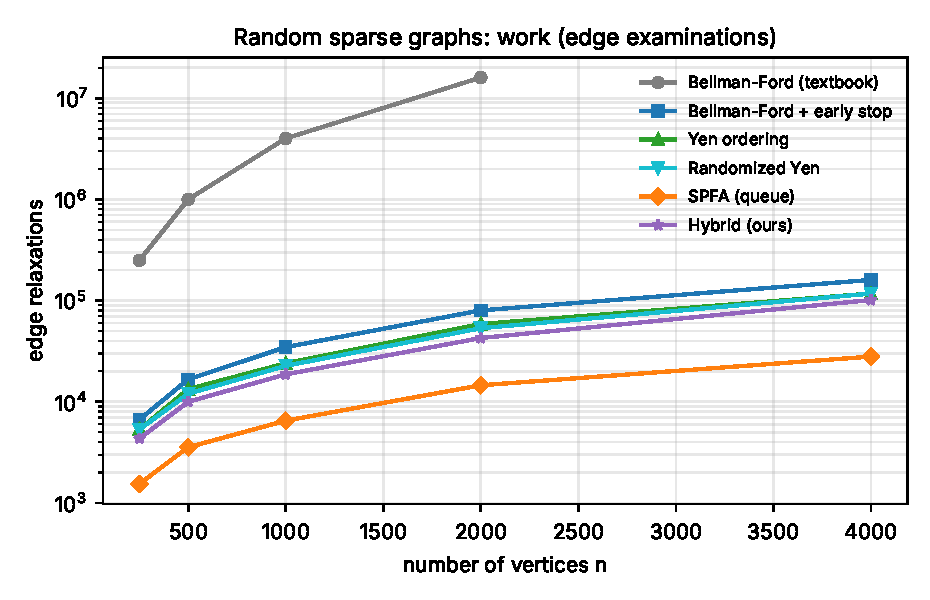
\includegraphics[width=0.49\linewidth]{random_relax.pdf}\hfill
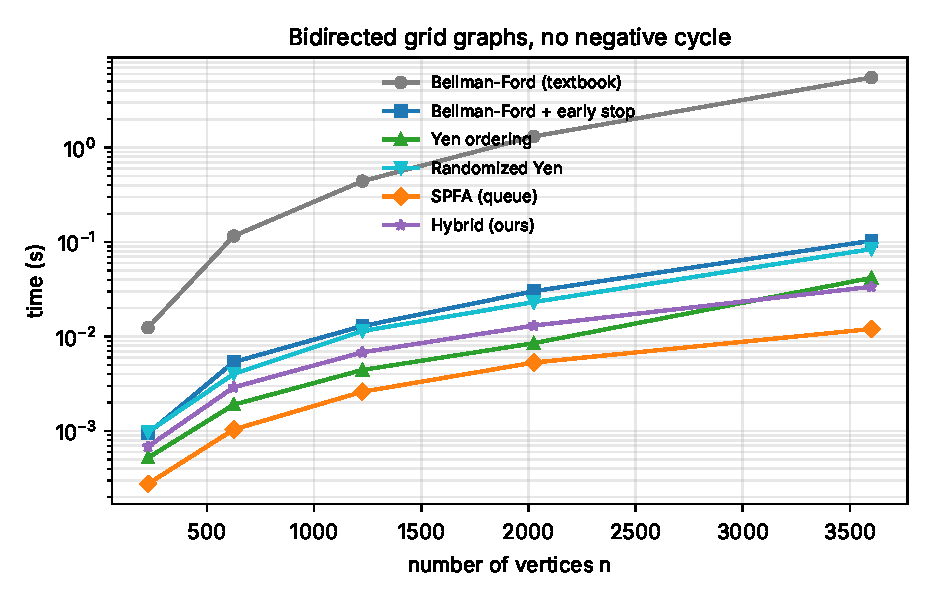
\includegraphics[width=0.49\linewidth]{grid_time.pdf}\\[4pt]
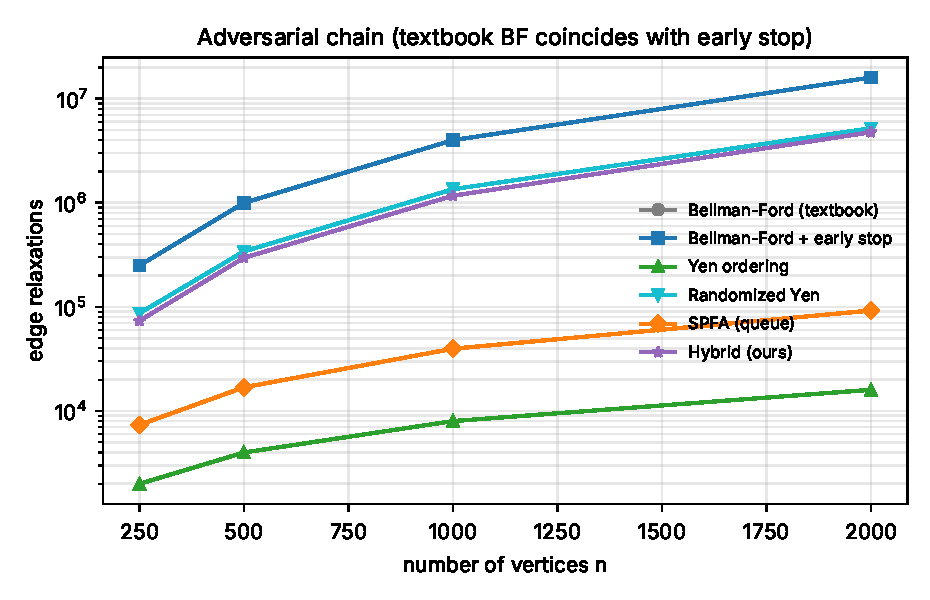
\includegraphics[width=0.49\linewidth]{chain_relax.pdf}\hfill
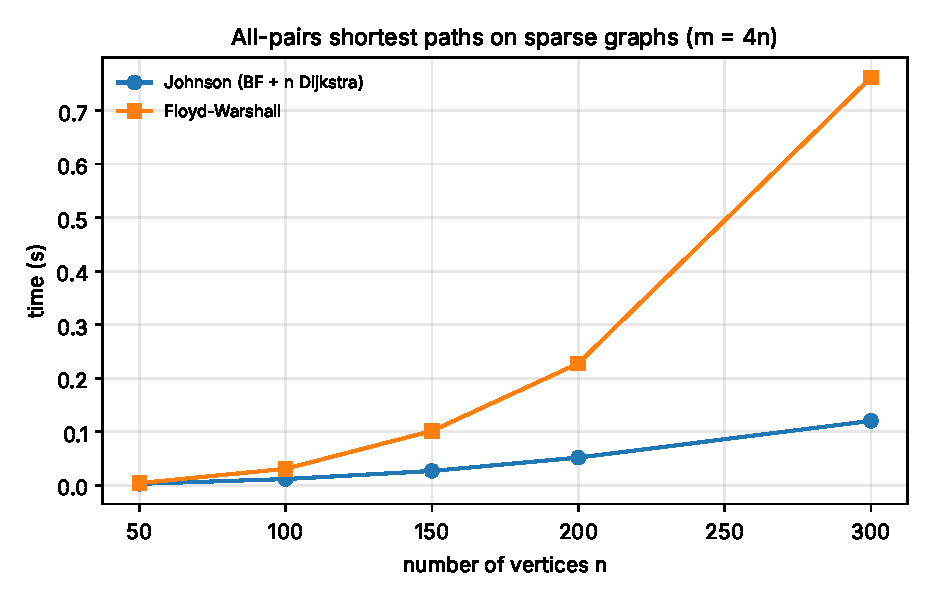
\includegraphics[width=0.49\linewidth]{apsp_time.pdf}
\caption{Graphs without negative cycles (log scale except APSP).}
\label{fig:noneg}
\end{figure}

\begin{table}[H]
\centering\small
\begin{tabular}{@{}lrrrrrr@{}}
\toprule
& \multicolumn{2}{c}{Random, $n=4000$} & \multicolumn{2}{c}{Grid, $n=3600$} & \multicolumn{2}{c}{Chain, $n=2000$}\\
\cmidrule(lr){2-3}\cmidrule(lr){4-5}\cmidrule(lr){6-7}
Algorithm & passes & time (s) & passes & time (s) & passes & time (s)\\
\midrule
Bellman--Ford (textbook) & $n$ & -- & 3600 & 5.526 & 2000 & 1.160\\
BF + early stop & 10.0 & 0.017 & 64.3 & 0.103 & 2000 & 1.233\\
Yen (identity order) & 7.3 & 0.021 & 10.7 & 0.042 & 2.0 & 0.005\\
Randomized Yen & 7.3 & 0.022 & 43.3 & 0.084 & 651 & 0.503\\
SPFA & -- & \textbf{0.010} & -- & \textbf{0.012} & -- & 0.019\\
Hybrid (BFS order) & \textbf{6.3} & 0.030 & \textbf{10.7} & 0.034 & 596 & 0.625\\
\bottomrule
\end{tabular}
\caption{Passes and running time (mean of 3 seeds). Textbook Bellman--Ford on random graphs was run up to $n=2000$, where it needed 1.48\,s against 0.0076\,s with early stopping.}
\label{tab:noneg}
\end{table}

\paragraph{Observations.}
\begin{enumerate}
\item \textbf{Early termination is the single most important practical fix.} On random graphs the hop depth is tiny, so early stopping cuts the work of Bellman--Ford by roughly $200\times$ at $n=2000$ ($1.6\times10^7$ vs.\ $8\times10^4$ relaxations). The $\Theta(nm)$ bound is a worst case that random inputs rarely approach.
\item \textbf{Ordering matters.} Yen-style passes need far fewer passes than plain Bellman--Ford whenever the ranking agrees with the direction of shortest paths. On grids, the BFS ranking of the hybrid needs about 11 passes against 64 for early-stop Bellman--Ford and 43 for a random ranking, a $3\times$ speed-up. On the adversarial chain, randomized Yen used $651\approx n/3$ passes, matching the Bannister--Eppstein prediction, while the identity order (which happens to coincide with the chain) needs only 2.
\item \textbf{Limitation of the BFS ranking.} On the chain, distracting edges let BFS reach far vertices early, so the BFS order does not follow the shortest-path tree and the hybrid behaves like a random ranking (596 passes). This confirms that the hybrid's guarantee is Yen's $\lceil n/2\rceil$ bound, not a better one.
\item \textbf{SPFA is the fastest when no negative cycle exists}, touching each vertex only a few times (about $7n$ relaxations on random graphs), because it never re-scans vertices whose labels did not change.
\item \textbf{Johnson beats Floyd--Warshall on sparse graphs}: $6.3\times$ faster at $n=300$, with a gap that grows with $n$ ($O(nm\log n)$ vs.\ $\Theta(n^3)$).
\end{enumerate}

\subsection{Results with negative cycles}

\begin{figure}[H]
\centering
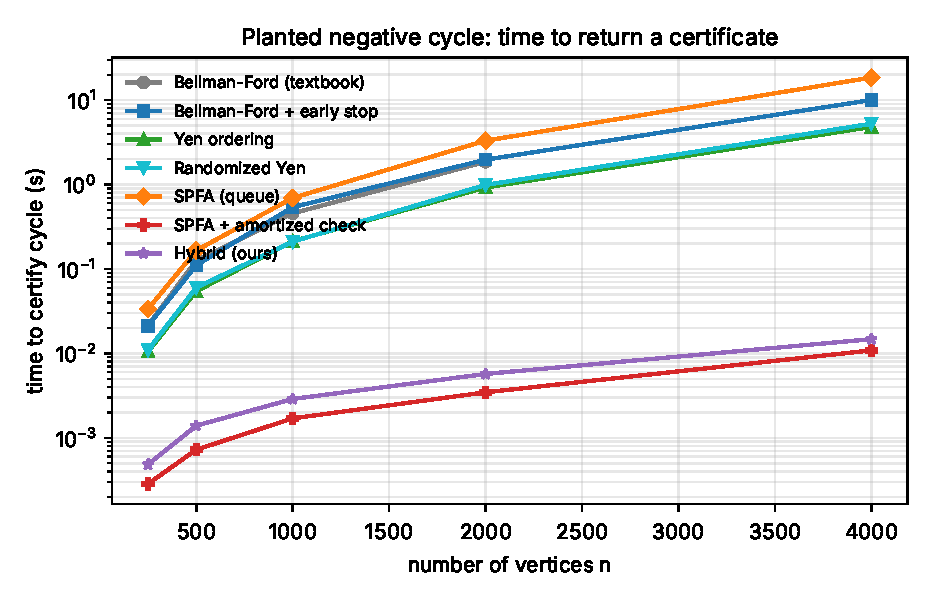
\includegraphics[width=0.49\linewidth]{negcycle_time.pdf}\hfill
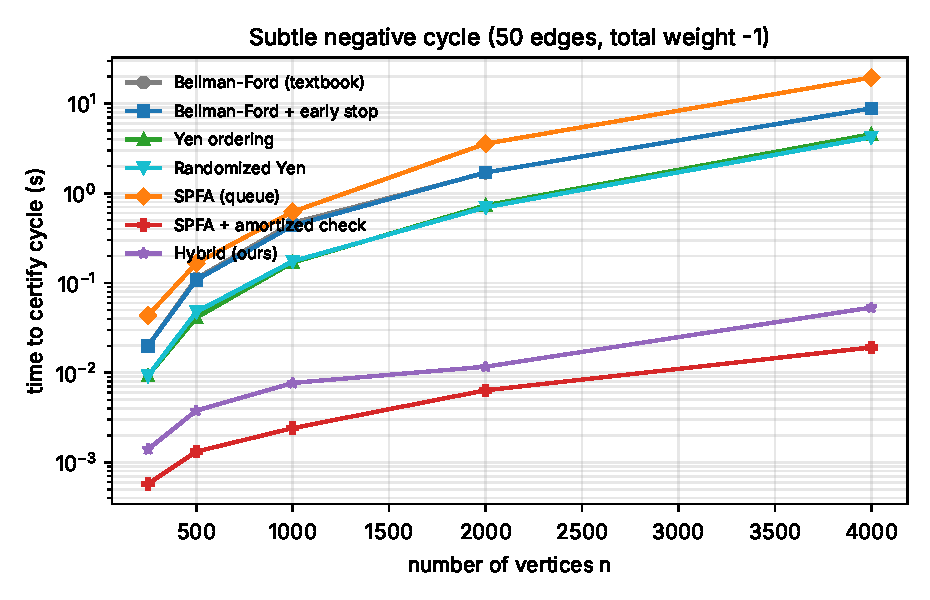
\includegraphics[width=0.49\linewidth]{subtle_time.pdf}
\caption{Time until a verified negative-cycle certificate is returned.}
\label{fig:neg}
\end{figure}

\begin{table}[H]
\centering\small
\begin{tabular}{@{}lrrrr@{}}
\toprule
& \multicolumn{2}{c}{Planted cycle, $n=4000$} & \multicolumn{2}{c}{Subtle cycle, $n=4000$}\\
\cmidrule(lr){2-3}\cmidrule(lr){4-5}
Algorithm & relaxations & time (s) & relaxations & time (s)\\
\midrule
BF + early stop & $6.4\times10^7$ & 10.025 & $6.4\times10^7$ & 8.850\\
Yen / randomized Yen & $3.2\times10^7$ & 4.819 & $3.2\times10^7$ & 4.205\\
SPFA (count $\ge n$) & $5.2\times10^7$ & 18.522 & $6.3\times10^7$ & 19.504\\
SPFA + amortized check & $2.2\times10^4$ & \textbf{0.011} & $3.9\times10^4$ & \textbf{0.019}\\
Hybrid (ours) & $1.6\times10^4$ & 0.015 & $2.3\times10^5$ & 0.053\\
\bottomrule
\end{tabular}
\caption{Negative-cycle detection (mean of 3 seeds).}
\label{tab:neg}
\end{table}

\paragraph{Observations.}
\begin{enumerate}
\item \textbf{Classical detection is the real bottleneck.} With a negative cycle, early stopping never fires, so Bellman--Ford pays the full $nm$ (4000 passes) and Yen pays $nm/2$ (2001 passes) every time. SPFA with the classic ``dequeued $n$ times'' rule is the \emph{slowest} of all, because vertices on the cycle are re-queued constantly.
\item \textbf{Predecessor-graph certificates change the picture.} Periodic $G_\pi$ checks (\cref{lem:predcycle}) return a verified cycle after a handful of passes. The hybrid needed 1 pass on planted cycles and 14 passes on the subtle cycle at $n=4000$, $167$--$670\times$ faster than early-stop Bellman--Ford. SPFA with amortized checks was fastest overall, about $460\times$ faster than Bellman--Ford on the subtle instance.
\item \textbf{The cost of checking is small.} When there is no negative cycle, the hybrid's BFS preprocessing and per-pass $O(n)$ search add a constant-factor overhead (about $1.4\times$ over Yen on random graphs) (random graphs, \cref{tab:noneg}) that is outweighed elsewhere by the benefit of early certificates.
\end{enumerate}


%======================================================================
\section{Conclusion}


Negative edge weights rule out Dijkstra's greedy method, and the possibility of negative cycles forces an algorithm either to compute distances or to produce a certificate that no distances exist. We formalised this problem, proved the correctness of Bellman--Ford, its early-terminating, Yen-ordered and queue-based variants, and Johnson's reweighting, and analysed their complexity.

Our main findings are:
\begin{itemize}
\item In theory, all classical label-correcting methods are stuck at $O(nm)$; ordering tricks only improve the constant (Yen: $1/2$, random ranking: $1/3$ in expectation).
\item In practice, the $O(nm)$ worst case is rarely reached \emph{unless a negative cycle is present}. Early termination and SPFA make the cycle-free case fast, but classical cycle detection always pays the full $\Theta(nm)$.
\item Predecessor-graph certificates, which we proved to be always negative cycles, fix this: checking them at amortized $O(1)$ cost per relaxation turned detection from seconds into milliseconds (up to $670\times$ faster in our experiments) with no false positives.
\item Our hybrid (BFS-ordered Yen passes, early stopping, certificate checks) is never worse than Yen's $\lceil n/2\rceil+1$ passes, gave a $3\times$ improvement over early-stop Bellman--Ford on grids and a $167$--$670\times$ improvement for cycle detection, but did not help when the BFS order disagrees with the shortest-path tree.
\item Beating $O(nm)$ \emph{asymptotically} requires fundamentally new ideas: scaling (Goldberg, $O(\sqrt n\,m\log W)$), low-diameter decompositions with randomized recursion (Bernstein--Nanongkai--Wulff-Nilsen and Bringmann--Cassis--Fischer, near-linear for integer weights), and, for real weights, Fineman's negative-vertex neutralisation ($\Ot(mn^{8/9})$, now $\Ot(mn^{4/5})$).
\end{itemize}
In short, the most effective practical recipe is ``label-correcting plus early termination plus amortized certificate checks'', while the theoretical frontier has moved to near-linear randomized algorithms whose practical value is still to be established.


%======================================================================
\section{Gaps and Future Directions}

\begin{enumerate}
\item \textbf{Deterministic near-linear time.} All near-linear negative-weight SSSP algorithms (BNW, BCF) are randomized. Almost-linear deterministic bounds ($m^{1+o(1)}$) follow from recent deterministic min-cost-flow algorithms, but these rely on heavy continuous-optimization machinery. A deterministic, combinatorial $\Ot(m\log W)$ algorithm remains open.
\item \textbf{Real weights.} For arbitrary real weights the best bounds ($\Ot(mn^{8/9})$, then $\Ot(mn^{4/5})$) are still far from near-linear. Whether real-weight SSSP can be solved in $\Ot(m)$, or even $O(m\sqrt n)$, is a major open question, and no matching conditional lower bound is known.
\item \textbf{Removing logarithmic factors.} Even for integers, BCF pays roughly $\log^2 n\log(nW)$ over linear. Closing the gap to $O(m\log W)$ or $O(m+n\log n)$ (Dijkstra's bound) is open.
\item \textbf{Practicality of the new algorithms.} The near-linear algorithms have large constants and complex recursion. Experimental studies comparing them with tuned Bellman--Ford and SPFA variants (such as our hybrid) on realistic inputs are scarce; an engineered implementation is a natural next step for this project.
\item \textbf{Better orderings.} Our experiments show that the vertex ordering in Yen-style passes matters a lot (BFS order vs.\ random). An open practical question is how to choose orderings adaptively (for example, re-ranking by the current shortest-path tree) while keeping worst-case guarantees, and how to combine them with Bannister--Eppstein randomization to get both a good expected bound and good typical behaviour.
\item \textbf{Dynamic, parallel and distributed settings.} Maintaining distances under edge updates with negative weights, and parallel algorithms with low depth and near-linear work, remain active areas; Bellman--Ford's inherent $n$ rounds is also the bottleneck in distributed (CONGEST) models.
\item \textbf{Faster negative-cycle detection and extraction.} Detecting a negative cycle is as hard as SSSP in the worst case, but returning a \emph{minimum-mean} or \emph{shortest} negative cycle quickly, or certifying absence in sublinear time on structured graphs, are open directions with direct applications (arbitrage, constraint solving).
\end{enumerate}

%======================================================================
\appendix
\section{Implementation and Reproducibility}

The code is in the \texttt{src/sssp} package of the project folder:
\begin{itemize}
\item \texttt{core.py}: graph structure, result object, predecessor-graph cycle search (\cref{lem:predcycle});
\item \texttt{algorithms.py}: Bellman--Ford (textbook and early stop), Yen, randomized Yen, SPFA (classic and with amortized checks), the hybrid, Dijkstra, Johnson and Floyd--Warshall;
\item \texttt{generators.py}: graph families used in the experiments;
\item \texttt{tests/test\_sssp.py}: 25 \texttt{pytest} tests comparing every algorithm against Floyd--Warshall on 720 random graphs (with and without negative cycles), verifying that every returned cycle is a real, reachable, negative cycle, and checking the Yen pass bound;
\item \texttt{experiments/benchmark.py}: reproduces all tables and figures; run it with \texttt{python experiments/benchmark.py}.
\end{itemize}

\section{Contribution of Group Members}
\begin{center}
\begin{tabular}{@{}lp{10.5cm}@{}}
\toprule
\textbf{Member} & \textbf{Contribution}\\
\midrule
Pragun Kathuria (2410110237) & Problem formulation, Bellman--Ford, early termination and correctness proofs; overall integration of report and code\\
Amitoj Oberoi (2410110046) & Johnson's algorithm, reweighting proof, Floyd--Warshall baseline and APSP experiments\\
Tanvi Pandey (2410110356) & Yen and randomized Yen orderings, SPFA, complexity analysis and comparison tables\\
Vishnu Sriram (2410110629) & Survey of scaling and near-linear algorithms (Goldberg, BNW, BCF, Fineman), gaps and future directions, benchmarking\\
\bottomrule
\end{tabular}
\end{center}

%======================================================================
\begin{thebibliography}{99}\small
\bibitem{bellman} R.~Bellman. On a routing problem. \emph{Quarterly of Applied Mathematics}, 16(1):87--90, 1958.
\bibitem{ford} L.~R.~Ford Jr. Network flow theory. RAND Corporation, Paper P-923, 1956.
\bibitem{moore} E.~F.~Moore. The shortest path through a maze. In \emph{Proc.\ Int.\ Symposium on the Theory of Switching}, 1959.
\bibitem{dijkstra} E.~W.~Dijkstra. A note on two problems in connexion with graphs. \emph{Numerische Mathematik}, 1:269--271, 1959.
\bibitem{yen} J.~Y.~Yen. An algorithm for finding shortest routes from all source nodes to a given destination in general networks. \emph{Quarterly of Applied Mathematics}, 27:526--530, 1970.
\bibitem{johnson} D.~B.~Johnson. Efficient algorithms for shortest paths in sparse networks. \emph{Journal of the ACM}, 24(1):1--13, 1977.
\bibitem{tarjan} R.~E.~Tarjan. Shortest paths. Technical report, AT\&T Bell Laboratories, 1981.
\bibitem{gabow} H.~N.~Gabow and R.~E.~Tarjan. Faster scaling algorithms for network problems. \emph{SIAM Journal on Computing}, 18(5):1013--1036, 1989.
\bibitem{goldberg} A.~V.~Goldberg. Scaling algorithms for the shortest paths problem. \emph{SIAM Journal on Computing}, 24(3):494--504, 1995.
\bibitem{cg} B.~V.~Cherkassky and A.~V.~Goldberg. Negative-cycle detection algorithms. \emph{Mathematical Programming}, 85:277--311, 1999.
\bibitem{cgr} B.~V.~Cherkassky, A.~V.~Goldberg and T.~Radzik. Shortest paths algorithms: theory and experimental evaluation. \emph{Mathematical Programming}, 73:129--174, 1996.
\bibitem{be} M.~J.~Bannister and D.~Eppstein. Randomized speedup of the Bellman--Ford algorithm. In \emph{Proc.\ ANALCO}, pp.\ 41--47, 2012.
\bibitem{cklpgs} L.~Chen, R.~Kyng, Y.~P.~Liu, R.~Peng, M.~Probst Gutenberg and S.~Sachdeva. Maximum flow and minimum-cost flow in almost-linear time. In \emph{Proc.\ FOCS}, 2022.
\bibitem{bnw} A.~Bernstein, D.~Nanongkai and C.~Wulff-Nilsen. Negative-weight single-source shortest paths in near-linear time. In \emph{Proc.\ FOCS}, 2022.
\bibitem{bcf} K.~Bringmann, A.~Cassis and N.~Fischer. Negative-weight single-source shortest paths in near-linear time: now faster! In \emph{Proc.\ FOCS}, 2023.
\bibitem{fineman} J.~T.~Fineman. Single-source shortest paths with negative real weights in $\Ot(mn^{8/9})$ time. In \emph{Proc.\ STOC}, 2024.
\bibitem{hjq} Y.~Huang, C.~Jin and K.~Quanrud. Faster single-source shortest paths with negative real weights via proper hop distance. In \emph{Proc.\ SODA}, 2025.
\bibitem{clrs} T.~H.~Cormen, C.~E.~Leiserson, R.~L.~Rivest and C.~Stein. \emph{Introduction to Algorithms}, 4th ed. MIT Press, 2022.
\end{thebibliography}

\end{document}
